\documentclass[12pt]{article}
\usepackage{amssymb, amsmath}
\usepackage{fancyhdr,lastpage}
\usepackage{amsmath,amsfonts,amssymb}
\usepackage{graphicx}
\usepackage{stix}
\usepackage{enumitem}
\usepackage{listings}
\tolerance 10000
\headheight 0in
\headsep 0in
\evensidemargin 0in
\oddsidemargin \evensidemargin
\textwidth 6.5in
\topmargin .25in
\textheight 8.7in

\usepackage{listings}
\usepackage{color}
 
\definecolor{codegreen}{rgb}{0,0.6,0}
\definecolor{codegray}{rgb}{0.5,0.5,0.5}
\definecolor{codepurple}{rgb}{0.58,0,0.82}
\definecolor{backcolour}{rgb}{0.95,0.95,0.92}
 
\lstdefinestyle{mystyle}{
    backgroundcolor=\color{backcolour},   
    commentstyle=\color{codegreen},
    keywordstyle=\color{magenta},
    numberstyle=\tiny\color{codegray},
    stringstyle=\color{codepurple},
    basicstyle=\footnotesize,
    breakatwhitespace=false,         
    breaklines=true,                 
    captionpos=b,                    
    keepspaces=true,                 
    numbers=left,                    
    numbersep=5pt,                  
    showspaces=false,                
    showstringspaces=false,
    showtabs=false,                  
    tabsize=2
}

\lstset{style=mystyle}

\newcommand{\CC}{{\mathbb C}}
\newcommand{\QQ}{{\mathbb Q}}
\newcommand{\RR}{{\mathbb R}}
\newcommand{\ZZ}{{\mathbb Z}}
\newcommand{\NN}{{\mathbb N}}
\newcommand{\FF}{{\mathbb F}}


\newcommand{\Zerobold}{{\boldsymbol 0}}
\newcommand{\Onebold}{{\boldsymbol 1}}
\newcommand{\xbold}{{\boldsymbol x}}

\newcommand{\mfrak}{{\mathfrak m}}

\newcommand{\Acal}{{\mathcal A}}
\newcommand{\Ncal}{{\mathcal N}}
\newcommand{\Pcal}{{\mathcal P}}
\newcommand{\Qcal}{{\mathcal Q}}

\newcommand{\sqbinom}[2]{\genfrac{[}{]}{0pt}{}{#1}{#2}}
\newcommand{\angbinom}[2]{\genfrac{\langle}{\rangle}{0pt}{}{#1}{#2}}

\newcommand{\qddx}{(d/dx)_{q}}

%\newcommand{\pfcl}{\emph{Proof of claim}}
\newenvironment{proof}{\paragraph{Proof: }}{\hfill$\blacksquare$}



\def\multiset#1#2{\ensuremath{\left(\kern-.3em\left(\genfrac{}{}{0pt}{}{#1}{#2}\right)\kern-.3em\right)}}


\DeclareMathOperator{\des}{des}
\DeclareMathOperator{\maj}{maj}
\DeclareMathOperator{\ev}{ev}
\DeclareMathOperator{\Hom}{Hom}
\DeclareMathOperator{\trace}{tr}
\DeclareMathOperator{\inv}{inv}

\newtheorem{problem}{Problem}%[section]

\begin{document}

\begin{center}
{\bf Julio Soldevilla}
\\
{\bf EECS 504 Winter 2018 --- Problem Set 1}
\end{center}

\begin{problem}
\normalfont
Problem 1
\end{problem}

\begin{proof}
\begin{enumerate}
\item  For this problm we can begin by just substituting the points into the equation $w\left[ \begin{matrix} x' \\ y' \\ 1\end{matrix} \right] = \left[ \begin{matrix} h_{11} & h_{12} & h_{13} \\ h_{21} & h_{22} & h_{23} \\ h_{31} & h_{32} & 1 \end{matrix} \right] \left[\begin{matrix} x \\ y \\1 \end{matrix}\right]$. If we do this, we end up having n matrices of the form \begin{equation} w\left[ \begin{matrix} x_i' \\ y_i' \\ 1\end{matrix} \right] = \left[ \begin{matrix} h_{11} & h_{12} & h_{13} \\ h_{21} & h_{22} & h_{23} \\ h_{31} & h_{32} & 1 \end{matrix} \right] \left[\begin{matrix} x_i \\ y_i \\1 \end{matrix}\right]\quad \text{for } i = 1,...,n\end{equation} which we can rewrite to have the following matrices: \begin{equation} \left[ \begin{matrix} 0 \\ 0 \\ 0 \end{matrix} \right] = \left[ \begin{matrix} x_i h_{11} + y_ih_{12} + h_{13} - wx_i' \\ x_i h_{21} + y_ih_{22} + h_{23} - wy_i' \\ x_i h_{31} + y_ih_{32} + 1 - w \end{matrix}\right]\quad \text{for } i = 1,...,n \end{equation}. Recall that in this problem we know the points $\{(x_i,y_i\}$ and $\{(x_i', y_i'\}$ but don't know the matrix with entries $h_{ij}$. This is nothing more than a giant system of equations and so we can rewrite more conveniently by considering the matrix $X = \left[ \begin{matrix} \frac{h_{11}}{w}\\ \frac{h_{12}}{w} \\ \frac{h_{13}}{w} \\ \frac{h_{21}}{w} \\ \frac{h_{22}}{w} \\ \frac{h_{23}}{w} \\ \frac{h_{31}}{w} \\ \frac{h_{32}}{w} \\ \frac{1}{w}\end{matrix} \right]$ which is the matrix we want to find, setting the matrix of known output values $Y = \left[ \begin{matrix} x_1' \\ y_1' \\ 1 \\ x_2' \\ y_2' \\ 1 \\ \vdots x_n' \\ y_n' \\ 1 \end{matrix} \right]$ and finally setting the matrix $$A = \left[\begin{matrix} x_1 & y_1 & 1 & 0 & 0& 0 & 0 & 0 & 0 \\ 0 & 0 & 0 & x_1 & y_1 & 1 & 0 & 0 & 0 \\ 0 & 0& 0 & 0 & 0 & 0 & x_1 & y_1 & 1 \\ x_2 & y_2 & 1 & 0 & 0& 0 & 0 & 0 & 0 \\ 0 & 0 & 0 & x_2 & y_2 & 1 & 0 & 0 & 0 \\ 0 & 0& 0 & 0 & 0 & 0 & x_2 & y_2 & 1 \\ \vdots & \vdots & \vdots & \vdots & \vdots & \vdots & \vdots & \vdots & \vdots \\ x_n & y_n & 1 & 0 & 0& 0 & 0 & 0 & 0 \\ 0 & 0 & 0 & x_n & y_n & 1 & 0 & 0 & 0 \\ 0 & 0& 0 & 0 & 0 & 0 & x_n & y_n & 1\end{matrix}\right]$$. THen, with this equations, we can reformulate the affine transformation estimation to minimize the standard least squares problem $$\min \|Ax - y\|_2^2$$ with the matrices $A$, $x$ and $y$ given above. \\

However, it seems in the formulation above we could still do some simplification, since we don't really care about the value of $w$ and we have a way of getting rid of it. Particularly, we can take equation 2 above and take the last entry. This entry tells us that $x_i h_{31} + y_ih_{32} + 1 -w = 0 \implies w =x_i h_{31} + y_ih_{32} + 1 \text{ for } i = 1,...,n$. Substituting thisv alue of $w$ into th erows above, we find that we have the relationships $x_i h_{11} + y_i h_{12} + h_{13} - x_i'x_i h_{31} - x_i'y_ih_{32} = -x_i'$ and $x_ih_{21} + y_ih_{22} + h_{23} -y_i'x_ih_{31} -y_i'y_ih_{32} = -y_i'$. This equations capture the same information as the formulation above but is just presented differently because we represented differently the relations represented the value $w$. Thus, we can rewrite this equation in matrix form again by considering the following matrices $X' = \left[\begin{matrix} h_{11} \\ h_{12} \\ h_{13} \\ h_{21} \\ h_{22} \\ h_{23} \\ h_{31} \\ h_{32} \end{matrix}\right]$ which is the matrix of unkowns that we want to find to find the homography transformation matrix, the matrix $Y' = \left[\begin{matrix} -x_1' \\ -y_1'\\-x_2' \\ -y_2' \\ -x_3' \\ -y_3'\\ \vdots\\-x_n' \\ -y_n'\end{matrix}\right]$ and finally the matrix $A' = \left[\begin{matrix} x_1 & y_1 &1 & 0& 0 & 0 & -x_1'x_1 & -x_1'y_1 \\ 0 & 0& 0 & x_1 & y_1 & 1  & -y_1'x_1 & -y_1'y_1 \\ x_2 & y_2 & 1 & 0& 0 & 0 & -x_2'x_2 & -x_2'y_2 \\0 & 0& 0 & x_2 & y_2 & 1 & -y_2'x_2 & -y_2'y_2\\ \vdots & \vdots & \vdots & \vdots & \vdots & \vdots & \vdots & \vdots \\ x_n & y_n &1 & 0& 0 & 0 & -x_n'x_n & -x_n'y_n \\ 0 & 0& 0 & x_n & y_n & 1 & -y_n'x_n & -y_n'y_n\end{matrix}\right]$. With these matrices, we can again reformulate the problem as the standard least-squares problem and just try to minimize $$\min\|A'x' - y'\|_2^2$$ with the matrices given in the second reformulation.

\item In any case of the reformulations above, we need to solve the least squares problem $\min \|Ax - y\|_2^2 = \min (Ax-y)^T (Ax-y)$. In this case, we will just the second set of matrices we found above. Recall that in this case the matrix $x'$ is the matrix $\left[\begin{matrix} h_{11} \\ h_{12} \\ h_{13} \\ h_{21} \\ h_{22} \\ h_{23} \\ h_{31} \\ h_{32} \end{matrix}\right]$ and so when taking a partial derivative with respect to $x_i$, we are taking with respect to the variable of entry $x_i$ in this matrix. To solve this, let $e = (Ax -y)$, then the problem to solve is $\min e^Te$ which we can do by taking the first derivative of this expression, setting it equal to 0 and solving for it. Letting $f(x) = e^Te$ we have that $f'(x) = 2 \frac{\partial e}{\partial x_i}e = 0 \stackrel{1}{\implies} c_i^T(Ax - y) = 0$ for all $i = 1,...,n$ where $c_i$ are the columns of matrix $A$ and $\frac{\partial e}{\partial x_i} = c_i$ and this derivative comes just from writing out the product $Ax-y$ and then differentiating every row and concatenating the resulting columns. Hence we have that the first derivative implies $c_i^T(Ax- y) = 0$, then concatenating for taking all the derivatives of the rows of the expression $Ax-y$ with respect to all the $x_i$ we have the expression $A^T(Ax - y) = 0 \implies A^TAx - A^Ty = 0 \implies A^TAx = A^Ty \implies x = (A^TA)^{-1}A^Ty$, and so this is the result to the estimation problem from above. \\

I claim we need $8$ points (counting both $x_i$ and $y_i$) to obtain a unique solution, so we require $4$ pairs of points. I think this is the answer because we want to determine the 8 entries $h_{ij}$ in the transformation matrix. TO do this, we need to solve the system of equations with 8 equations given in the second formulation of the problem above. Since with 4 points this matrix becomes a square matrix, we have that the rank of the matrix is 8 with no relationships between the rows or columns, namely it would have full rank and so it would be invertible, allowing us to find a unique solution by just finding the inverse of $A$. Notice that this if we consider less than 3 pairs of points, then the matrix might not be full rank.

\item In the following we present the code used to solve the problem. 

\lstinputlisting[language=Matlab]{hw1p1.m}

Now, we show the image that results as output of the code above in figure 1. It is important to notice that the points obtained for the correspondences are $XY1 = \left[\begin{matrix} 1134.65 & 517.9 \\ 1134.7 & 589.9 \\ 1614.2 & 561.9 \\ 966.9 & 314.2 \end{matrix}\right]$ and $XY2 = \left[\begin{matrix} 615.2638 & 613.8468 \\ 415.4766 & 689.7660 \\ 863.000 & 629.8298 \\ 231.6723 & 426.0468 \end{matrix}\right]$ and with these vectors we get the transformation matrix $H = \left[\begin{matrix} 0.9147 & 0.0949 & -707.4416 \\ -0.0633 & 0.9968 & 175.5697 \\ -0 & -0 & 1 \end{matrix} \right]$:

\begin{figure}[h]
\begin{center}
\centering
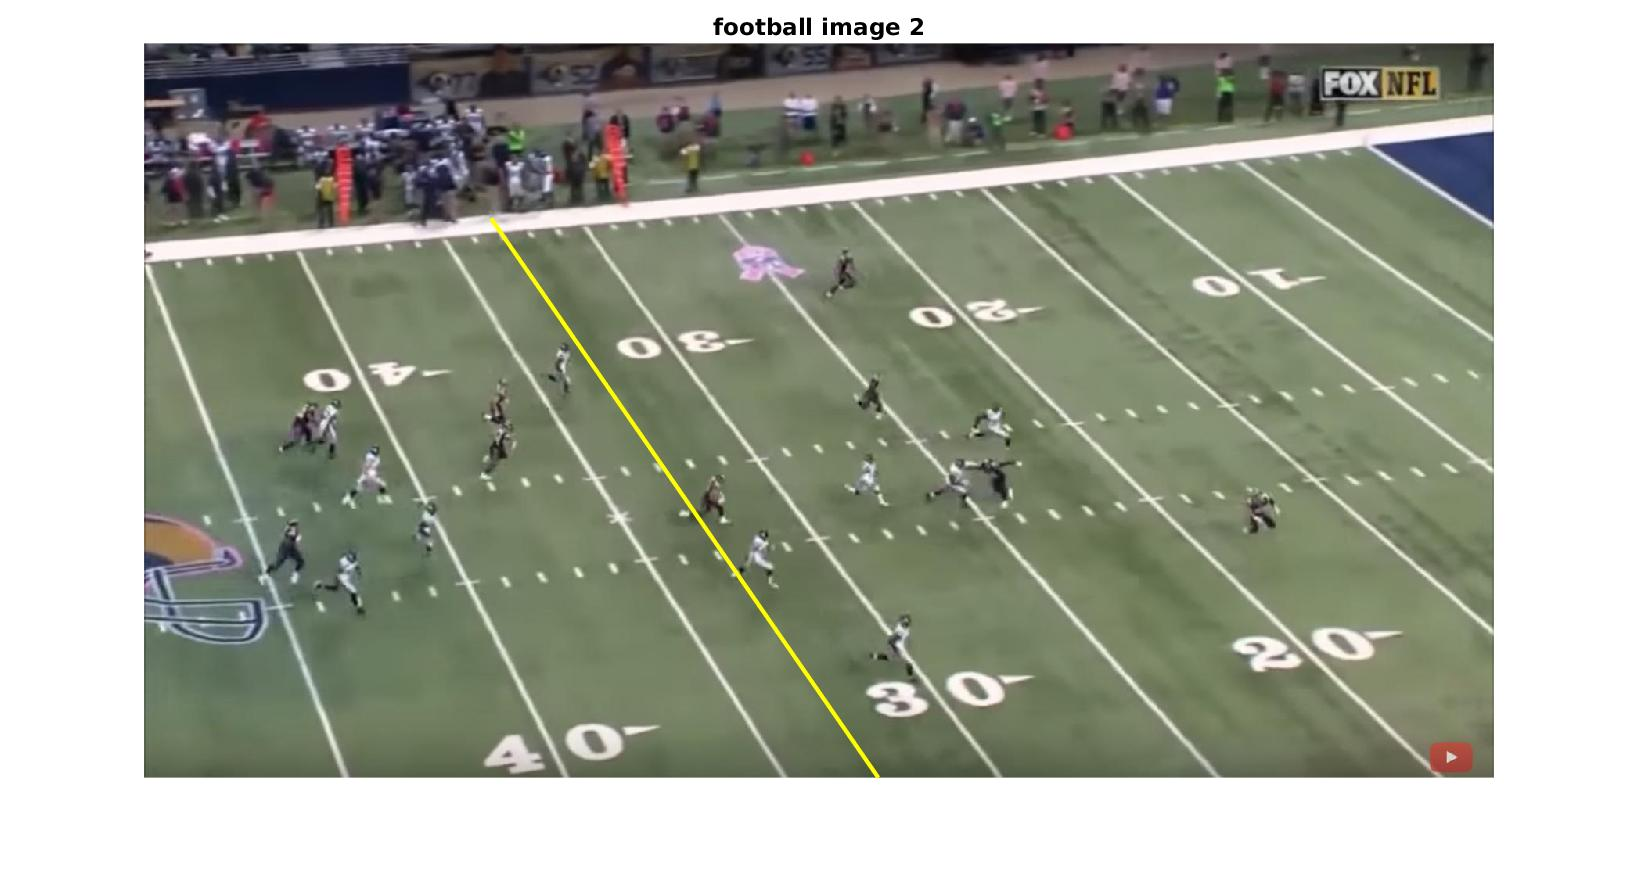
\includegraphics[scale=0.3]{problem1_output.jpg}
\caption{This is the image that we get as output after running the code above using the points XY1 and XY2}
\label{fig:mesh1}
\end{center}
\end{figure}

To finish, we also present the original image with the 33 yard line in figure 2:

\begin{figure}[h]
\begin{center}
\centering
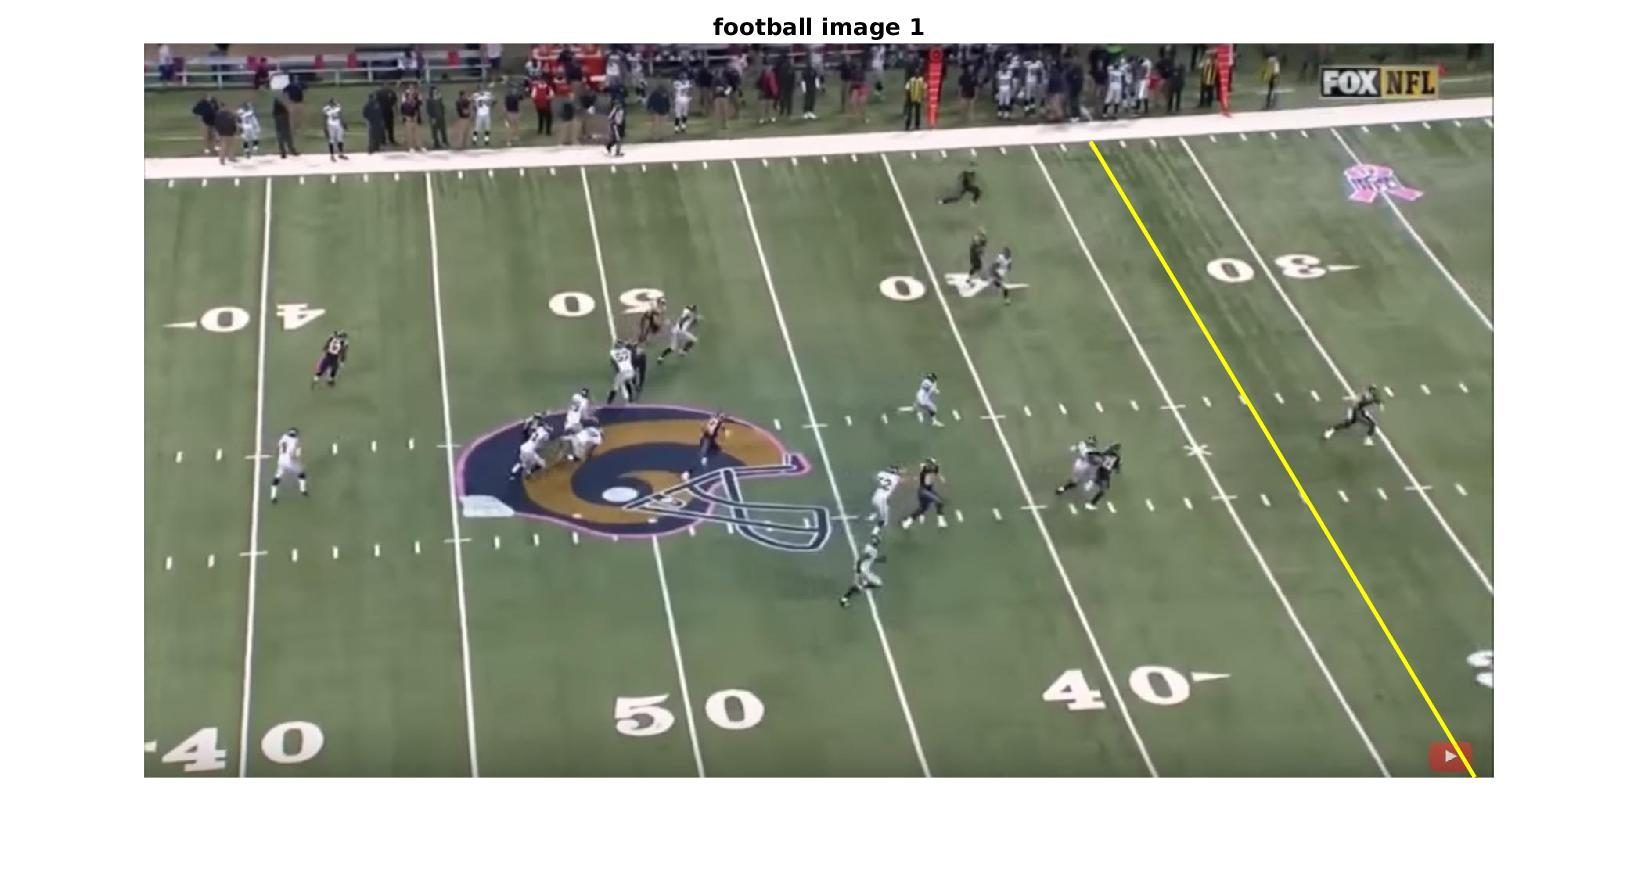
\includegraphics[scale=0.3]{problem1_orig_im.jpg}
\caption{Original image with 33 yard line, no transformation.}
\label{fig:mesh1}
\end{center}
\end{figure}

\end{enumerate}
\end{proof}

\pagebreak

\begin{problem}

Problem 2

\end{problem}

\begin{proof}
The issue with the given model on vertical lines is that in this case we are trying to compute the vertical distance of the points to the line, but that is impossible in this case since the line is vertical and there is no vertical distance between the data points and the line we compute (additionally, the slope of such line is $m = \infty$ and so we cannot do the substraction required in the least squares problem). So, to avoid this issue (and any issue with horizontal lines too), first we can reparameterize the line as $Ax + By + C = 0$. With this reformulation, we can also reformulate the least squares problem to be $E(A,B,C) = \sum_{i=1}^n(Ax_i + By_i + C)^2$, so the least squares problem would be 

\begin{equation*}
\begin{aligned}
& \underset{A,B,C}{\text{minimize}}
& & \sum_{i=1}^n(Ax_i + By_i + C)^2  \\
& \text{subject to}
& & A^2 + B^2 = 1
\end{aligned}
\end{equation*}

where we have the last constraint to ensure that we are not considering repeated lines, or lines that are the same but the coefficients are just multiplied by some constant, i.e. lines with coefficients $A,B,C$ and then lines with coefficients $2A,2B,2C$. Furthermore, we can interpret the equation $Ax_i + By_i + C = d_i$ as the distance between the lime we want estimate and the points we have, then the minimization problem is to minimize the sum of this distance with respect to all the points in the data set. Notice that this reformulation of the least squares problem solves the issue with vertical and horizontal lines, since when we have vertical lines, we just set the coefficient of $Y$ to be $0$ and we will be able to minimize the horizontal distances between the points and the line we are estimating, namely minimize the expression $\sum_{i=1}^n (Ax_i + C)^2$ and when we have horizontal lines, the coefficient of $X$ will just turn out to be $0$, and we will be able to minimize the horizontal distances between the points and the line we are estimating, namely minimize the expression $\sum_{i=1}^n(By_i + C)^2$. Thus this reformulation solves the problem with the least squares estimation of horizontal and vertical lines. Now, we can also do a matrix formulation of the minimization problem by rewriting the line equation as $Ax +By + C = 0 \iff [\begin{matrix} A & B & C \end{matrix}] \left[ \begin{matrix} x_1 & x_2 & \dots & x_n \\ y_1 & y_2 & \dots & y_n \\ 1 & 1 & \dots & 1\end{matrix} \right] = 0$. THen, the minimization problem would be $\min_{A,B,C} \left\|[\begin{matrix} A & B & C \end{matrix}] \left[ \begin{matrix} x_1 & x_2 & \dots & x_n \\ y_1 & y_2 & \dots & y_n \\ 1 & 1 & \dots & 1\end{matrix} \right]\right\|_2^2 = \min_{A,B,C} \left([\begin{matrix} A & B & C \end{matrix}] \left[ \begin{matrix} x_1 & x_2 & \dots & x_n \\ y_1 & y_2 & \dots & y_n \\ 1 & 1 & \dots & 1\end{matrix} \right] \right)^T\left([\begin{matrix} A & B & C \end{matrix}] \left[ \begin{matrix} x_1 & x_2 & \dots & x_n \\ y_1 & y_2 & \dots & y_n \\ 1 & 1 & \dots & 1\end{matrix} \right]\right)$. Now, in this case, if we try to find the solution of this problem by finding the first derivative and setting this equation equal to $0$, letting $e = [\begin{matrix} A & B & C \end{matrix}] \left[ \begin{matrix} x_1 & x_2 & \dots & x_n \\ y_1 & y_2 & \dots & y_n \\ 1 & 1 & \dots & 1\end{matrix} \right]$ we end up having that such derivative $f'(x) = 2 \frac{\partial e}{\partial x_i}e = 2A [\begin{matrix} A & B & C \end{matrix}] \left[ \begin{matrix} x_1 & x_2 & \dots & x_n \\ y_1 & y_2 & \dots & y_n \\ 1 & 1 & \dots & 1\end{matrix} \right] =  0 $. However, if we try to solve this (therefore getting the pseudo inverse expression) we just end up having that $\left[\begin{matrix} X \\ Y \\ 1\end{matrix}\right] = 0$, which is not a solutio to this problem. This issue when obtaining the solution to the least squares via the first derivative implies that we \textbf{cannot} use the pseudo-inverse to solve the minimization problem.
 \end{proof}

\begin{problem}
Problem 3
\end{problem}

\begin{proof}
\begin{enumerate}

\item I claim that both $A$ and $B$ will observe the reflection at point $x$ with the same strength. First of all notice that the lambertian model of reflectance $R(x) = \rho \mathcal(x)^T n(x)$ is a formula that contains information about the surface normal with $n(x)$, about the direction of incident light source $\mathcal{L}(x)$, hence it contains no information of the strength that someone will observe the reflection and thus we can concldue that the radiance emitted from a Lambertian surface is not a function of outgoing direction, hence since the formula for the Lambertian surface has no information about the strength of the reflection, it must be that both $A$ and $B$ perceive the strength of the reflection at x equally.

\item One major drawback of Lambertian surface model is that it only captures diffuse characteristics of the surface, but not ambient lighting, specular reflections or other more complex radiometric functions. One object in the real world whose reflectance is not welll modeled by the Lambertian model is a mirror or glass.

\end{enumerate}
\end{proof}

\begin{problem}
Problem 4
\end{problem}

\begin{proof}
Here we present the code of the function mydemosaic.m

\lstinputlisting[language=Matlab]{mydemosaic.m}

The original image we are considering for this problem is the following one, in figure 3:

\begin{figure}[h]
\begin{center}
\centering
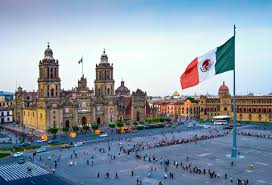
\includegraphics[scale=1]{CDMX.jpg}
\caption{Original image considered for this problem.}
\label{fig:mesh1}
\end{center}
\end{figure}

Then, the gray-scaled image obtained from the Bayer filter function is seen in figure 4 and in figure 5 we see the other result from the bayer filter function. 

\begin{figure}[h]
\begin{center}
\centering
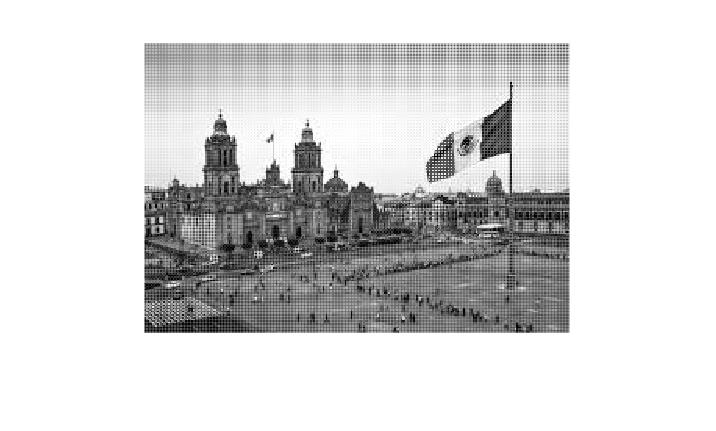
\includegraphics[scale=0.50]{CDMX_filtered_gray.jpg}
\caption{Gray-scaled image obtained from Bayer filter function.}
\label{fig:mesh1}
\end{center}
\end{figure}

\begin{figure}[h]
\begin{center}
\centering
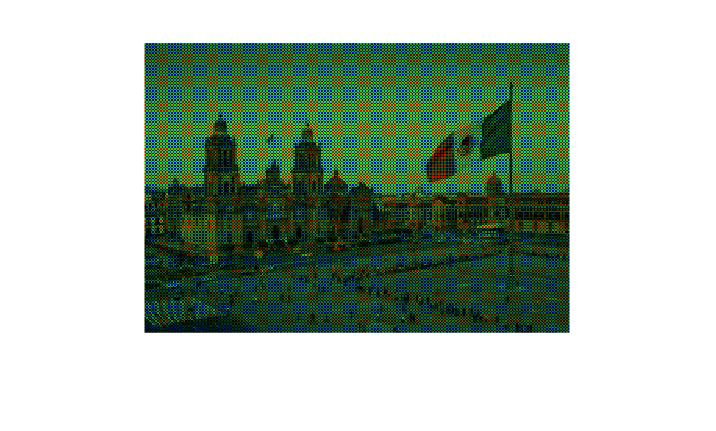
\includegraphics[scale=0.50]{CDMX_bayer_filter.jpg}
\caption{Image obtained from bayer filter (non-gray scale).}
\label{fig:mesh1}
\end{center}
\end{figure}

Finally, this is the image we get as output from the mydemosaic.m function we implemented, we see such image in figure 6.

\begin{figure}[h]
\begin{center}
\centering
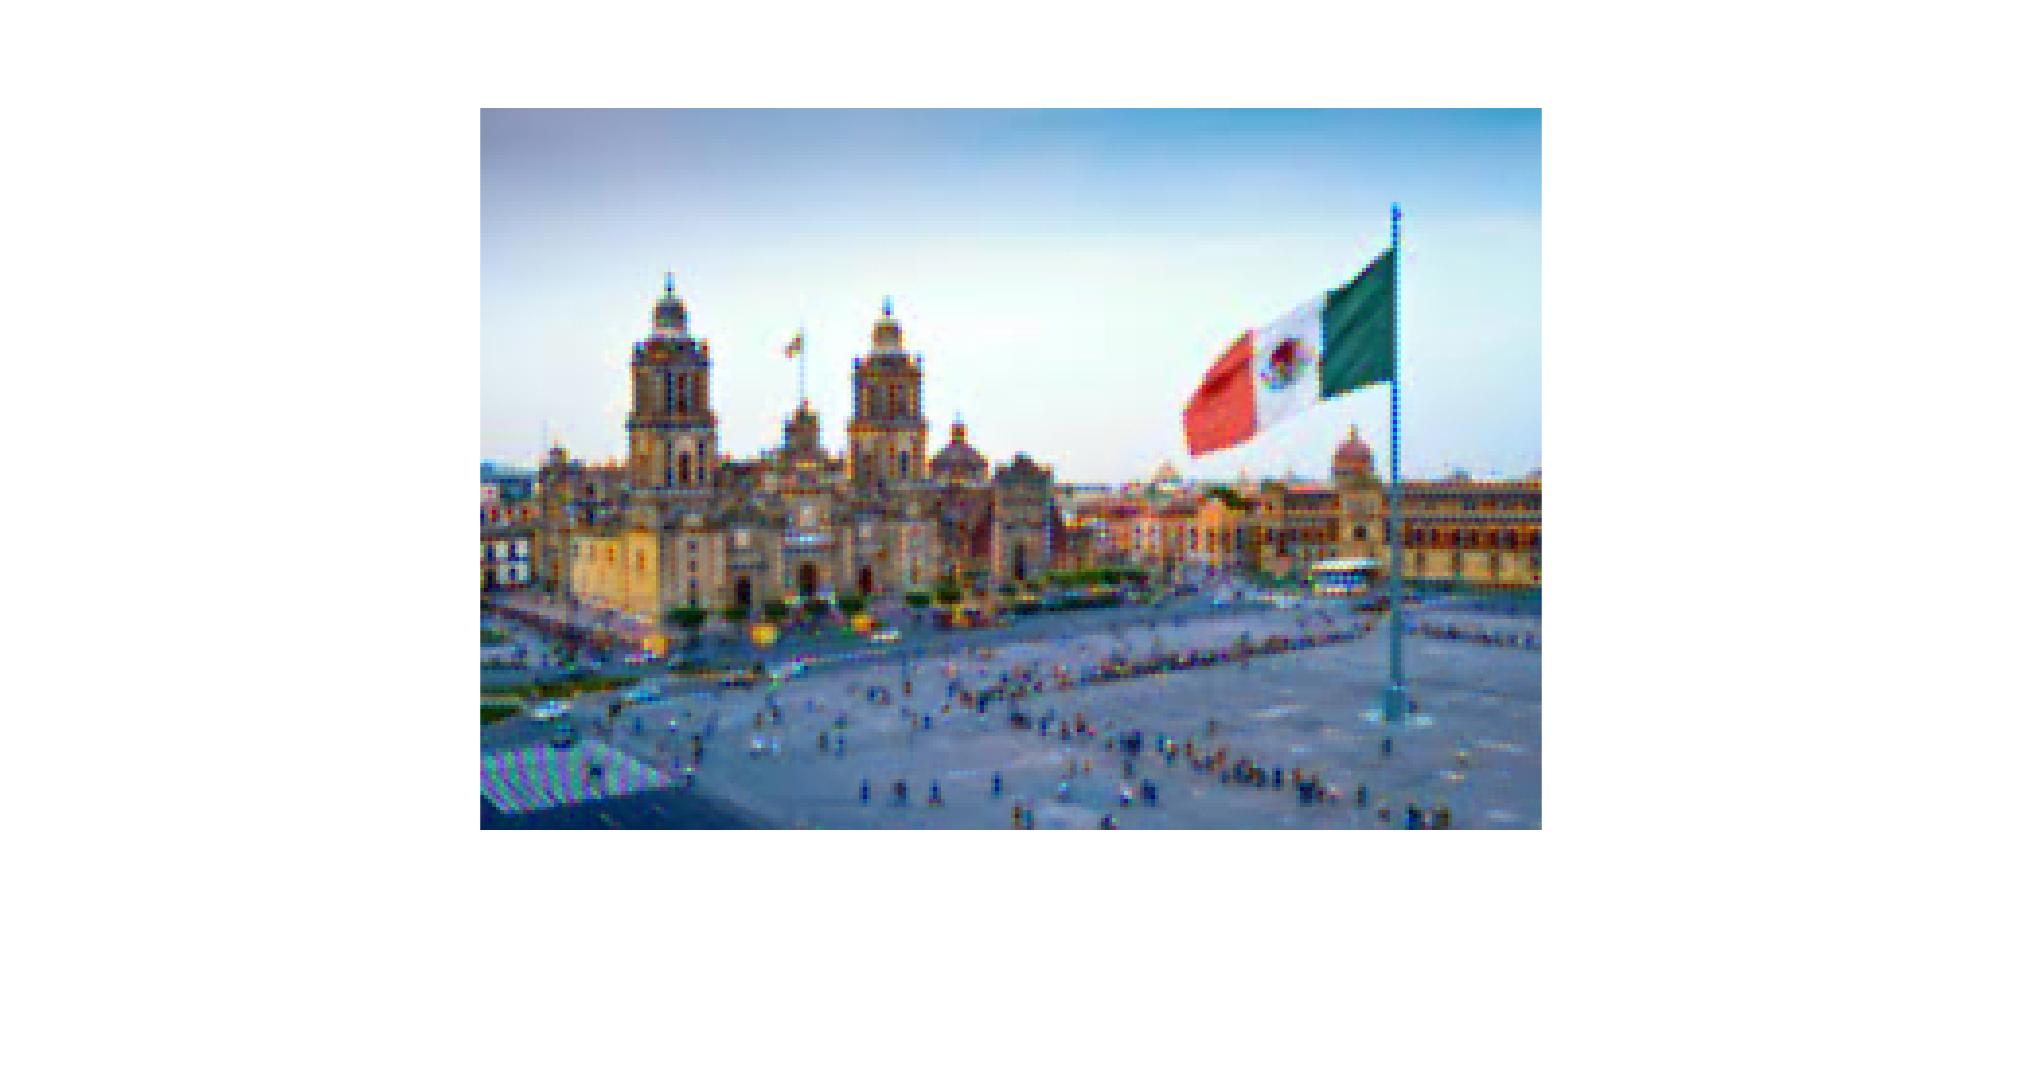
\includegraphics[scale=0.25]{CDMX_mydemosaic.jpg}
\caption{Output image from function mydemosaic.}
\label{fig:mesh1}
\end{center}
\end{figure}





\end{proof}

\end{document}